%preámbulo
\documentclass[12pt,oneside,FLEQN]{report}
\usepackage{amssymb,amsthm,amsmath,enumerate,graphicx,tabularx}
\usepackage[utf8]{inputenc}
\usepackage[hidelinks]{hyperref}
\usepackage[spanish]{babel}
\usepackage[rflt]{floatflt}
\usepackage{multicol}
\usepackage{tcolorbox, empheq}
\tcbuselibrary{skins,breakable,listings,theorems}
\usepackage{tikz,tkz-tab}
\usetikzlibrary{matrix,arrows, positioning,shadows,shadings,backgrounds,calc, shapes, tikzmark}
\usepackage{subfigure}
\usepackage{caption}
\usepackage[a4paper]{geometry}
\geometry{top=1.5cm, bottom=1.5cm, left=3cm, right=3cm}
\usepackage{ragged2e}
\newcommand{\marcar}[3]{\tikz[overlay,remember picture,baseline=-2pt] \node[circle,#1,draw,text=black, inner sep=1pt] (#2) { #3};}
\parindent=0cm
\usepackage{listings}
\hypersetup{
colorlinks=true,
linkcolor=black,
filecolor=magenta,
urlcolor=cyan,
citecolor=greenwhats
}
\usepackage[dvipsnames,table]{xcolor}
%\usepackage{lscape}
\usepackage{enumitem}
\definecolor{greenwhats}{RGB}{37, 211, 102}
\definecolor{gris}{rgb}{0.33, 0.41, 0.47}
\usepackage{fancyhdr}
\usepackage{natbib}
\usepackage{colortbl}
\usepackage{array,booktabs}
%\usepackage{pdflscape}
\usepackage{longtable}
\definecolor{codeturquoise}{RGB}{72,202,228}
\definecolor{codeyellow}{RGB}{255,170,51}
\definecolor{codepurple}{RGB}{255, 203, 242}
\definecolor{codegreen}{RGB}{149,213,178}
\definecolor{backcolour}{RGB}{73,80,87}
\definecolor{white}{RGB}{255,255,255}
\lstdefinestyle{estilochidori}{
backgroundcolor=\color{backcolour},
commentstyle=\color{codeyellow},
keywordstyle=\color{codeturquoise},
numberstyle=\tiny\color{codegreen},
stringstyle=\color{codepurple},
basicstyle=\ttfamily\footnotesize\color{white},
breakatwhitespace=false,
breaklines=true,
captionpos=b,
keepspaces=true,
numbers=left,
numbersep=5pt,
showspaces=false,
showstringspaces=false,
showtabs=false,
tabsize=2
}
\lstset{style=estilochidori}
\begin{document}
{
\fontfamily{qag}\selectfont
\begin{titlepage}
        \topmargin=0cm
        \centering

        {\bfseries\LARGE Universidad Autónoma de Querétaro \par}
        \vspace{1cm}
        {\scshape\Large  Facultad de Ingenier\'ia  \par}
        \vspace{2cm}
        \centering
        \begin{figure}[!h]
        \centering
                
\includegraphics[height=5cm]{Logouaq.png}
        \end{figure}
        \vspace{3cm}
        {\itshape\large Tarea 2: Métodos cerrados para ecuaciones de una variable\par}
        \vspace{3cm}
        {\Huge Análisis numérico \par}
        \vspace{2cm}
        {\Large Autor: \par}
        {\large J.A. Salinas Sánchez \par}
        {\large Febrero 2022 \par}
\end{titlepage}
\tableofcontents
\chapter{Introducción}
	Siguiendo con el hecho de que el análisis numérico surge de que existen expresiones matemáticas que son muy difíciles de resolver exactamente, o que aún se desconoce una manera de hacerlo; es fácil deducir que debe existir alguna ecuación de una sola variable que cumpla con este criterio. Lo cual es cierto, pues cualquier ecuación que contenga dos o más funciones de distinto tipo, o ambas trascendentes sobre su variable independiente; se vuelven indespejables, ya que siempre se aplicará una o más funciones a la variable. Un ejemplo es la ecuación $x=e^x$, porque, como se puede observar; nunca se conseguirá obtener una función explícita para x. Por otro lado, existe una gran variedad de funciones que, aunque sean perfectamente resolvibles vía analítica; son complicadas o tardadas de resolver. Un ejemplo podría ser cualquier raíz de orden mayor al 2.\\

	Por eso y más, se desarrolló una serie de algoritmos para poder encontrar soluciones numéricas a ecuaciones de una variable, sin importar cuál sea, y para comenzar, se verán los métodos cerrados. Los métodos cerrados para resolver ecuaciones de una variable, toman su nombre del hecho de que sólo pueden realizarse dentro de un intervalo cerrado definido por unos valores iniciales entre los cuales debe localizarse la raíz o , de otra forma, estos métodos nunca la encontrarán. Estos métodos son tres: el método gráfico, el método de bisección y el método de falsa posición. 
	\begin{enumerate}
		\item Método gráfico: consiste en realizar una gráfica de la función que represente a la ecuación original, dejando como variable independiente a la incógnita del problema, y así, ver la intersección de ésta con el eje de la variable independiente; obteniendo, así, una aproximación a la raíz de la ecuación.\\
			Como se puede observar, este método toma la naturaleza de ser un método cerrado, pues se debe conocer el intervalo donde se encuentra la respuesta al problema para poder verla al momento de hacer la gráfica.
		\item Método de bisección: este método consta de escoger un intervalo adecuado e ir dividiéndolo a la mitad, para luego tomar como nuevo intervalo, al subintervalo izquierdo o derecho del anterior, dependiendo del comportamiento de la función en dicho intervalo. Este método tiende a no estancarse; pero, por ser de fuerza bruta, tiende a ser ineficiente.
		\item Método de falsa posición: es similar al método anterior, pero se vuelve un poco más eficiente, ya que se va guiando a la respuesta, mediante una línea recta armada con los puntos de iteraciones anteriores; por lo que se puede ahorrar iteraciones en comparación del método de bisección.
	\end{enumerate}
\chapter{Método y resultados}
	\section{Método y pseudocódigo}
Como se pudo observar, tanto el método de bisección como el de falsa posición solamente difieren en un paso: definir el resultado provisional. Por tanto, el pseudocódigo será, en esencia,el mismo:
	\lstinputlisting{pseudo.txt}
	\section{Problemas}
	De lo visto en el apartado anterior, los siguientes códigos serán más o menos extensos dependiendo de los métodos solicidatos; no obstante, contendrán una o más secciones de lo expuesto en el pseudocódigo anterior, ya que, es literalmente el mismo código; pero con valores iniciales y funciones diferentes; además de más o menos métodos. Inclusive, las funciones programadas para cada uno de los métodos es casi la misma, como ya se dijo.
		\subsection{5.3}
		Determine las raíces reales de $f(x)=0.7x^5-8x^4+44x^3-90x^2+82x-25$:
		\begin{itemize}
			\item a: Gráficamente.
			\item b: Usando el método de bisección  con $E_{s}=10\%$. Utilice como valores iniciales xl=0.5 y xu=1.
			\item c: Realice el mismo cálculo que en b, pero con el método de la falsa posición y $E_{s}=0.2\%$.
		\end{itemize}
			\lstinputlisting{53.py}
		\begin{figure}[!h]
			\centering
				\subfigure[Método gráfico]{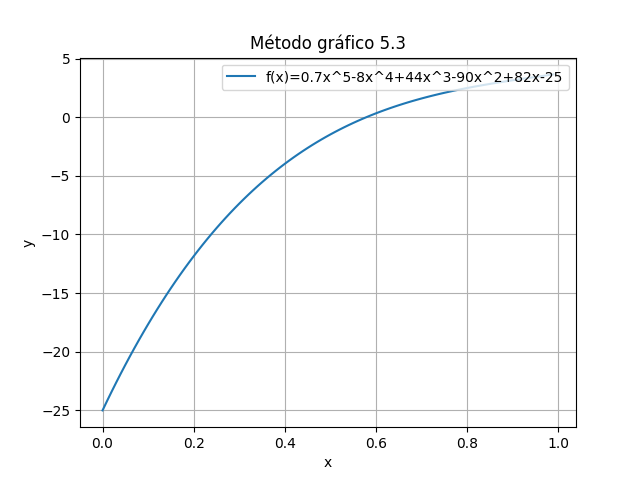
\includegraphics[scale=0.3]{53graph.png}}
				\subfigure[Error vs. iteraciones: bisección]{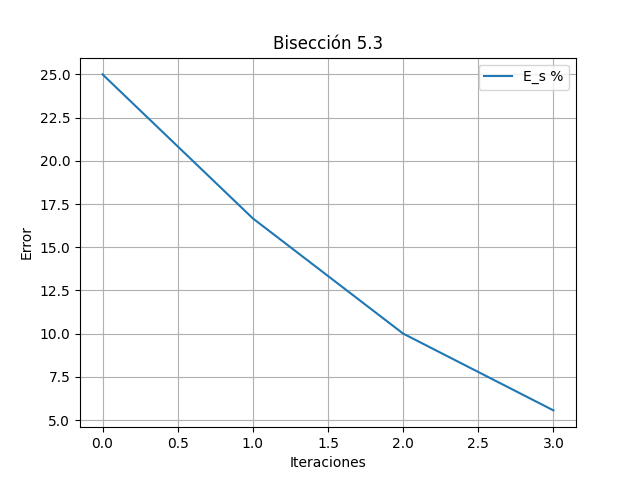
\includegraphics[scale=0.3]{53bis.png}}
				\subfigure[Error vs. iteraciones: falsa posición]{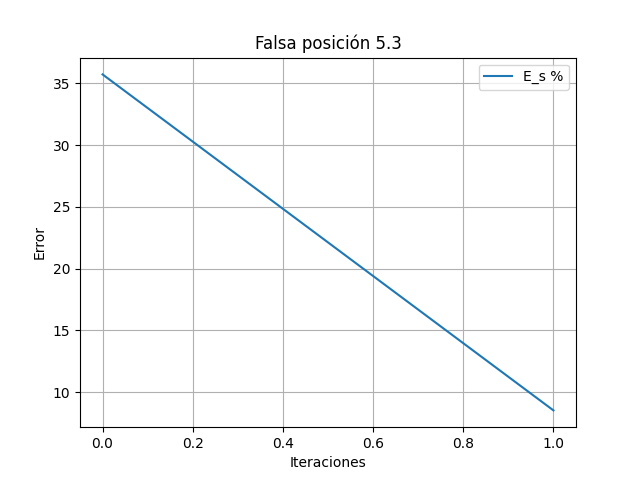
\includegraphics[scale=0.3]{53fp.png}}
		\end{figure}
		\subsection{5.11}
		Determine la raíz real de $x^3.5=80$:
		\begin{itemize}
			\item a: de manera analítica.
			\item b: con falsa posición con $E_{s}=2.5\%$.Haga elecciones iniciales de 2 a 5.
		\end{itemize}
			\lstinputlisting{511.py}
		\subsection{5.13}
		La velocidad v de un paracaidista que cae, está dada por:
		\begin{equation}
			v=\dfrac{gm}{c}\left(1-e^{-(c/m)t}\right)
		\end{equation}
		Donde g=9.81$m/s^2$, c=15$kg/s$, calcule la masa m de modo que la velocidad sea v=36$m/s$ en t=10s. Utilice el método de la falsa posición para determinas m a un nivel de $E_{s}=0.1\%$.
			\lstinputlisting{513.py}
		\subsection{5.15}
		Como se ilustra den la figura P5.15, la velocidad del agua v (m/s), en la descarga de un tanque cilíndrico a través de un tubo largo, se puede calcular como:
		\begin{equation}
			v=\sqrt{2gH}\tanh{\left(\dfrac{\sqrt{2gH}}{2L}t\right)}
		\end{equation}
		Determine la carga hidrostática H para obtener v=5m/s en 2.5s, con un tubo de 4m de largo. Hágalo gráficamente, por bisección y con posición falsa.Utilice xl=0 y xu=2 con un nivel de $E_{s}=1\%$.
			\lstinputlisting{515.py}
		\subsection{5.17}
		Suponga que el lector está diseñando un tanque esférico para almacenar agua para un poblado pequeño en un país en desarrollo (México xD). El volumen del líquido que puede contener se calcula con :
		\begin{equation}
			V=\pi h^2\dfrac{3R-h}{3}
		\end{equation}
		Donde V es el volumen [$m^3$], h es la profundidad de agua en el tanque (m), y R, el radio del tanque en metros.\\

		Si R=3m, ¿a qué profundidad debe llenarse el tanque de modo que contenga 30$m^3$?. Haga tres iteraciones con el método de falsa posición a fin de obtener la respuesta. Determine el error relativo aproximado después de cada iteración. Utilice 0 y R.
			\lstinputlisting{517.py}
	\section{Resultados}
	\begin{center}
		\begin{tabular}{|c|c|c|}
			\hline
			Problema&Bisección&Falsa posición\\
			5.3&0.59375&0.588017\\
			5.11&NO&3.44349\\
			5.13&NO&62.30246\\
			5.15&1.25&1.27\\
			5.17&NO&2.0268\\
			\hline
		\end{tabular}
	\end{center}
\chapter{Conclusiones}
\chapter{Referencias}
}
\end{document}
